\section{Theorie}
\label{sec:Theorie}

\subsection{Gekoppelte Schwingkreise} 
\label{sub:Gekoppelte Schwingkreise}


\begin{figure}

    \centering
    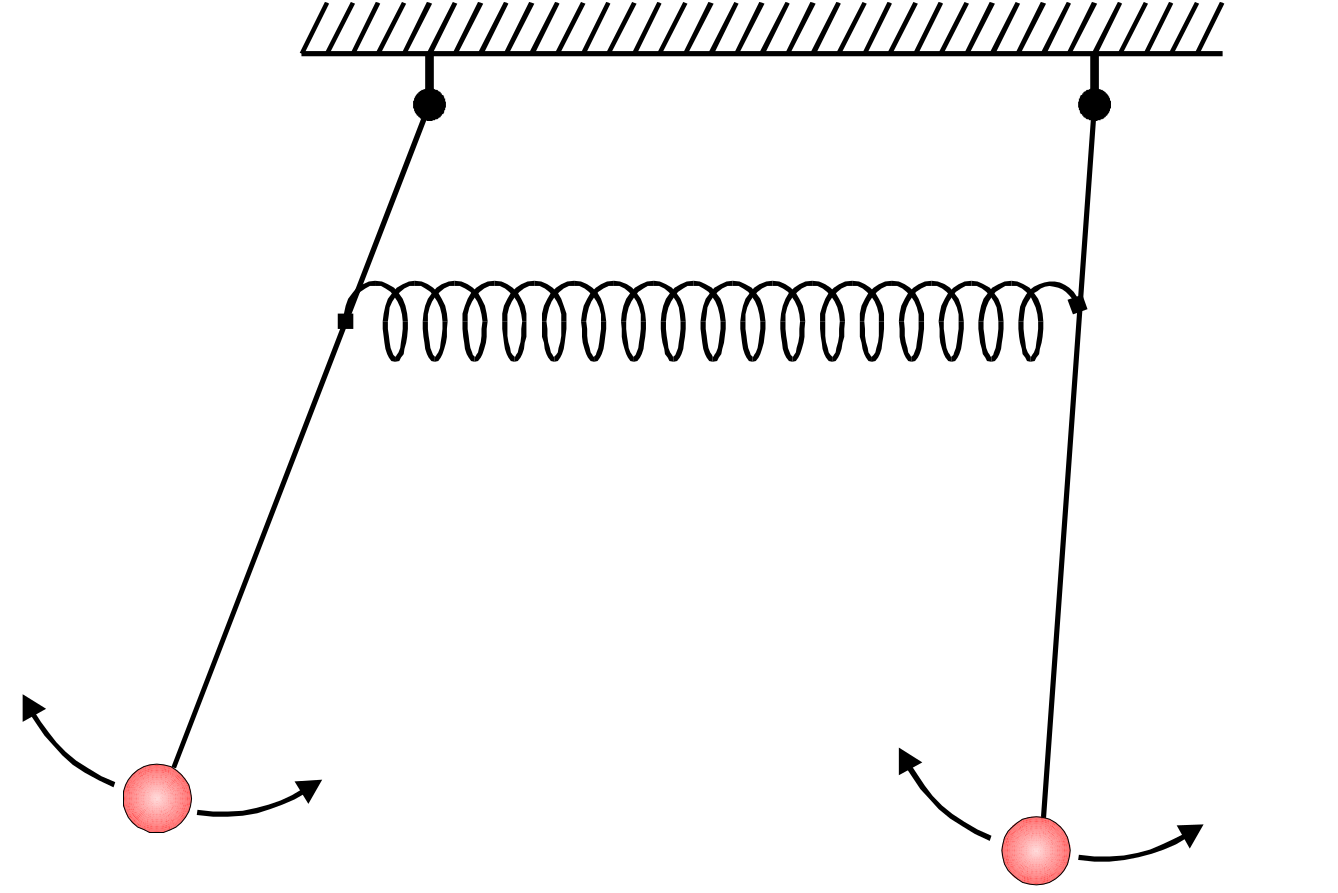
\includegraphics[height=6.0cm]{data/Bild1.png}
    \caption{Zwei gekoppelte Pendel.}
    \label{fig:bild1}
\end{figure}

Bei einem gekoppeltem Schwingkreis handelt es sich um zwei Schwingkreise, bei denen im Laufe der Schwingung
die Energie von einen in den anderen Schwingkreis übertagen werden kann. Ein einfachen Beispiel für ein gekoppeltes
System sind zwei Pendel, welche durch eine Feder miteinander verbunden sind. Veranschaulicht in Bild \ref{fig:bild1} dargestellt. Dabei dient die Feder als Medium für die hin- und herübertragung der Energie der einzelnen Pendel.
Auf diese Weise würde das System, bei Vernachlässigung von dissipativen Effekten, endlos weiter Schwingen.
In dem Versuch werden kapazitiv gekoppelte LC-Schwingkreise betrachtet, welche im Prinzip wie in Abbildung \ref{fig:bild2}
aufgebaut sind. Dabei sind die Kirchhoffschen Regeln wichtige Eigenschaften von elektrischen Schaltkreisen: 

1.  Die Summe der zufließenden Ströme in einem Knotenpunkt eines Stromkreises entspricht
    der Summe der abfließenden Ströme.

2.  Die Summe aller Spannungen innerhalb einer Masche eines geschlossenen Stromkreises
    ist null.


Im Folgenden ist zu beachten, dass die Spule $L$ in der Realität, wie im Erstazschaltbild dargestellt, zusätzlich zu ihrer Induktivität noch eine Kapazität
$C_\text{sp}$ hat. Die in den folgenden Formeln angegebene Kapazität $C$ setzt sich also aus $C_\text{kon} + C_\text{sp}$ = $C$ 
zusammen. 

\begin{figure}

    \centering
    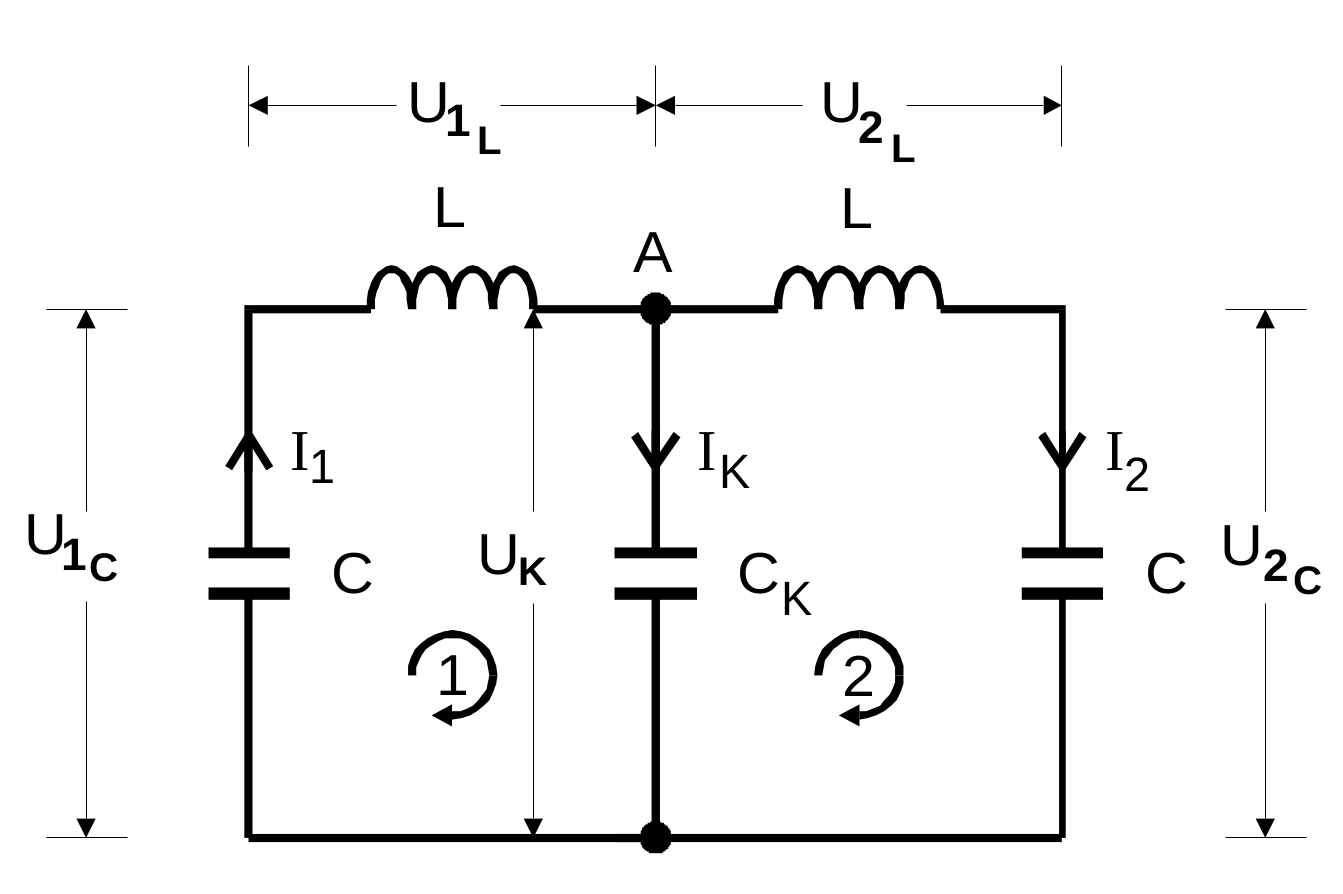
\includegraphics[height=6.0cm]{data/Bild2.png}
    \caption{Schaltbild zwei gekoppelter Schwingkreise.}
    \label{fig:bild2}
\end{figure}

Aus diesem System \ref{fig:bild2} lassen sich mit Hilfe der Kirchhoffschen Regeln und den Zusammenhängen
\begin{equation*}
    U_C=\frac{1}{C}\int I \, \symup{dt}
\end{equation*}
und
\begin{equation*}
    U_L=L\dot{I}
\end{equation*}
folgende homogene Differentialgleichungen aufstellen:
\begin{equation}
\label{eqn:diff1}
    L\dv[2]{(I_1+I_2)}{t}+\frac{1}{C}(I_1+I_2)=0 
\end{equation}
\begin{equation}
\label{eqn:diff2}
    L\dv[2]{(I_1-I_2)}{t}+\left(\frac{1}{C}+\frac{1}{C}\right)(I_1-I_2)=0 
\end{equation}

Die Lösung von \eqref{eqn:diff1} ist 
\begin{equation}
\label{eqn:l1}
    (I_1+I_2)(t)=(I_{1_0}+I_{2_0})\cos(\frac{t}{\sqrt{LC}})
\end{equation}
mit der Schwingungsfrequenz:
\begin{equation}
\label{eqn:frq1}
    \nu^+=\frac{1}{2\pi\sqrt{LC}}
\end{equation}

Die Lösung der Differentialgleichung \eqref{eqn:diff2} ergibt sich zu
\begin{equation}
\label{eqn:l2}
    (I_1-I_2)(t)=(I_{1_0}-I_{2_0})\cos(\frac{t}{\sqrt{L\left(\frac{1}{C}+\frac{2}{C_k}\right)^{-1}}})
\end{equation}
mit der Schwingungsfrequenz:
\begin{equation}
\label{eqn:frq2}
    \nu^-=\frac{1}{2\pi\sqrt{L\left(\frac{1}{C}+\frac{2}{C_k}\right)^{-1}}}
\end{equation}

Durch Addition und Subtraktion von \eqref{eqn:l1} und \eqref{eqn:l2} können die einzelnen Ströme durch
\begin{equation}
\label{eqn:I1}
    I_1(t)=\frac{1}{2}(I_{1_0}+I_{2_0})\cos(2\pi\nu^+t)+\frac{1}{2}(I_{1_0}-I_{2_0})\cos(2\pi\nu^-t)
\end{equation}
und 
\begin{equation} 
\label{eqn:I2}
    I_2(t)=\frac{1}{2}(I_{1_0}+I_{2_0})\cos(2\pi\nu^+t)-\frac{1}{2}(I_{1_0}-I_{2_0})\cos(2\pi\nu^-t)
\end{equation}
beschrieben werden.

Bei genauer Betrachtung der Gleichungen \eqref{eqn:I1} und \eqref{eqn:I2} lassen sich zwei besondere Spezialfälle erschließen.
Bei gleicher Amplitude und Phase ($I_{1_0}=I_{2_0}$) verhalten sich die Schwingkreise so, als wenn sie nicht gekoppelt wären, da sich die 
jeweilgen Ströme stets gegenseitig kompensieren. Bei gleicher Amplitude, aber entgegengesetzter Phase schwingen beide Schwingkreise mit 
der höheren Frequenz $\nu^-$ aus Gleichung \eqref{eqn:frq2}. Diese beiden Spezialfälle werden \enquote{Fundamentalschwingungen} des Systems genannt.

Bei Auslenkung von nur einem Schwingkreis $(I_{1_0}\neq 0,I_{2_0}=0)$ entstehen Schwebungen:
\begin{equation}
    I_1(t)=I_{1_0}\cos(\frac{1}{2}2\pi\left(\nu^++\nu^-\right)t)\cos(\frac{1}{2}2\pi\left(\nu^+-\nu^-\right)t)
\end{equation}
\begin{equation}
    I_2(t)=I_{1_0}\sin(\frac{1}{2}2\pi\left(\nu^++\nu^-\right)t)\sin(\frac{1}{2}2\pi\left(\nu^+-\nu^-\right)t)
\end{equation}

Die Frequenz der Schwebung ergibt sich zu $\nu_s=\nu^--\nu^+$, wobei das System mit der Frequenz
\begin{equation}
    \frac{1}{2}(\nu^++\nu^-)\approx \nu^+
\end{equation}
schwingt.

Ein Beispiel einer Schwebung ist schematisch in Bild \ref{fig:bild3} dargestellt.
\begin{figure}

    \centering
    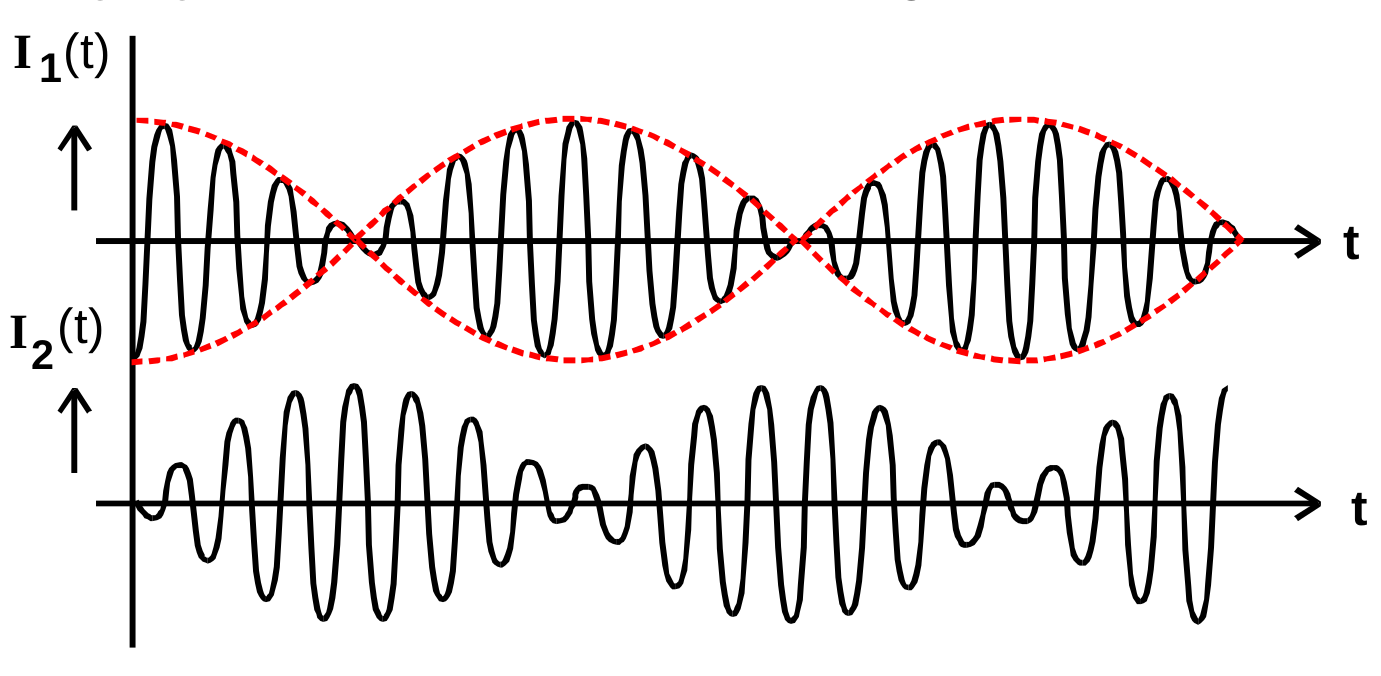
\includegraphics[height=6.0cm]{data/Bild3.png}
    \caption{Schematische Darstellung einer Schwebung.}
    \label{fig:bild3}
\end{figure}

Da in der Realität jede Spule auch eine gewisse Kapazität besitz, wird stellvertretend für diese Kapazität ein
virtueller Kondensator parallel zu der jeweilgen Spule geschaltet. Dies ist in Abbildung \ref{fig:bild7} dargestellt. 
Die Frequenzen $\nu^+$ und $\nu^-$ lassen sich dann über
\begin{equation}
    \nu^+=\frac{1}{2\pi\sqrt{L(C+C_{\text {sp}})}}
\end{equation}
\begin{equation}
    \nu^-=\frac{1}{2\pi\sqrt{L\left(\left(\frac{1}{C}+\frac{2}{C_k}\right)^{-1}+C_{\text {sp}}\right)}}
\end{equation}
bestimmen.
Die theoretische Anzahl der Maxima innerhalb einer Schwebungsperiode kann mit Hilfe der Gleichung
\begin{equation}
    n_t=\frac{\nu^++\nu^-}{2(\nu^--\nu^+)}
\end{equation}
berechnet werden.
\begin{figure}

    \centering
    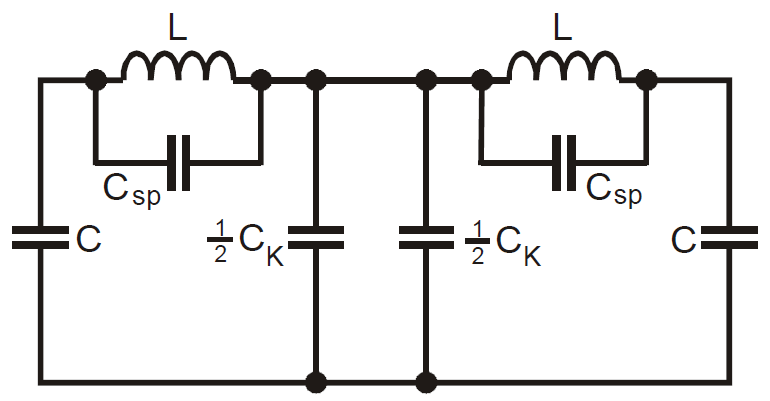
\includegraphics[height=6.0cm]{data/Bild7.png}
    \caption{Schaltbild eines Schwingkreises mit realen Spulen.}
    \label{fig:bild7}
\end{figure}

\subsection{angeregter Schwingkreis}

\begin{figure}

    \centering
    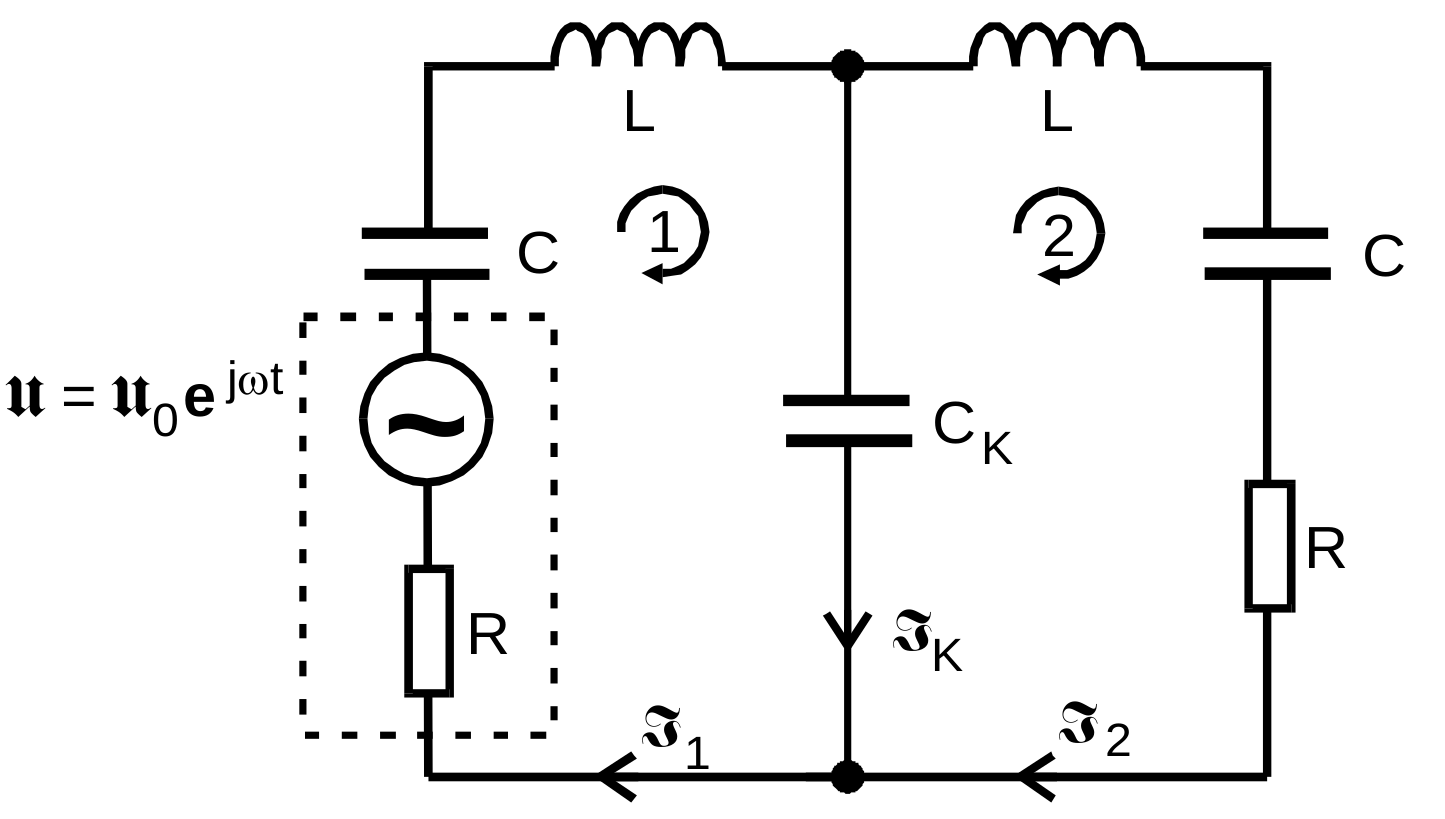
\includegraphics[height=6.0cm]{data/Bild4.png}
    \caption{Realer Schwingkreis mit anregendem Sinusgenerator.}
    \label{fig:bild4}
\end{figure}

Im folgenden wird die Theorie des frequenzabhängigen Stroms in einem gekoppelten Schwingkreis aufgeführt.
Im Allgemeinen lässt sich in der Realität kein absolut dämpfungsfreier Schwingkreis erzeugen. Desshalb sind die Schwingkreise in Schaltung \ref{fig:bild4}
mit jeweils einem ohmschen Widerstand versehen, um die realen Verluste zu simulieren. Bei Betrachtung der Schaltung \ref{fig:bild4} lassen sich folgende 
Gesetzmäßigkeiten ableiten:
\begin{equation}
    \left|I_2\right|=\left|U\right|\frac{1}{\sqrt{4\omega^2C_K^2R^2Z(\omega)^2+\left(\frac{1}{\omega C_K}-\omega C_KZ(\omega)^2+\omega R^2C_K\right)^2}}
\end{equation}
wobei $Z(\omega)$ als
\begin{equation}
    Z(\omega)\coloneq \omega L-\frac{1}{\omega}\left(\frac{1}{C}+\frac{1}{C_K}\right)
\end{equation}
definiert ist.

$I_2$ erreicht bei den Fundamentalfrequenzen $\omega^+$ und $\omega^-$ jeweils ein Maximum, welche sich über die Gleichungen
\begin{equation}
    \left|I_2(\omega^+)\right|=\frac{1}{R\sqrt{4+\frac{R^2C_K^2}{LC}}}
\end{equation}
und 
\begin{equation}
    \left|I_2(\omega^-)\right|=\frac{1}{R\sqrt{4+\frac{R^2C_K^2}{LC}}\left(1+\frac{C}{C_K}\right)}
\end{equation}
berechnen lassen, wobei  $\left|I_2(\omega^+)\right|$ und $\left|I_2(\omega^-)\right|$ zu
\begin{equation}
    \left|I_2(\omega^+)\right|\approx\left|I_2(\omega^-)\right|\approx \frac{1}{2R}
\end{equation}
genähert werden können.

%In knapper Form sind die physikalischen Grundlagen des Versuches, des Messverfahrens, sowie sämtliche für die Auswertung erforderlichen Gleichungen darzustellen. (Keine Herleitung)

%(eventuell die Aufgaben)

%Der Versuchsaufbau: Beschreibung des Versuchs und der Funktionsweise (mit Skizze/Bild/Foto)
